\documentclass[11pt]{article}
\usepackage{amssymb,amsmath,lmodern,slashed,cancel}
\usepackage{array}
\usepackage{bm}
\usepackage{graphicx}
\usepackage[hidelinks]{hyperref}
\usepackage[toc,page]{appendix}
\usepackage{footnote,url}
\usepackage{calc}
\usepackage{caption}
\usepackage{xspace}
\usepackage[export]{adjustbox}
\usepackage{subcaption}
\usepackage[margin=.5in,top=1in]{geometry}
\usepackage{fancyhdr}
\usepackage{float}
\renewcommand{\headrulewidth}{0.4pt}
\renewcommand{\footrulewidth}{0.4pt}
\newlength\dlf
\newcommand\alignboxed[2]{
  &
  \begingroup
  \settowidth\dlf{$\displaystyle #1$}
  \addtolength\dlf{\fboxsep+\fboxrule}
  \hspace{-\dlf}
  \boxed{#1 #2}
  \endgroup
}
\newcommand\numberthis{\addtocounter{equation}{1}\tag{\theequation}}
\newcommand{\ve}{\mathbf{v}}
\newcommand{\Se}{\mathbf{S}}
\newcommand{\kk}{\vec{k}}
\newcommand{\ue}{\bm{u}}
\newcommand{\sgn}{\text{sgn}}
\newcommand{\p}{\mathbf{p}}
\newcommand{\vr}{\mathbf{r}}
\newcommand{\pop}{\hat{p}}
\newcommand{\vq}{\mathbf{q}}
\newcommand{\x}{\vec{x}}
\newcommand{\xop}{\hat{x}}
\newcommand{\w}{\mathbf{w}}
\newcommand{\z}{\mathbf{z}}
\newcommand{\y}{\vec{y}}
\newcommand{\qq}{\vec{q}}
\newcommand{\tv}{\tilde{\ve}}
\newcommand{\vL}{\vec{L}}
\newcommand{\vS}{\vec{S}}
\newcommand{\vso}{\vec{S}^{(1)}}
\newcommand{\vst}{\vec{S}^{(2)}}
\newcommand{\so}{S^{(1)}}
\newcommand{\st}{S^{(2)}}
\newcommand{\vJ}{\vec{J}}
\newcommand{\vl}{\vL}
\newcommand{\vj}{\vJ}
\newcommand{\vjo}{\vec{J}^{(1)}}
\newcommand{\vjt}{\vec{J}^{(2)}}
\newcommand{\jo}{J^{(1)}}
\newcommand{\jt}{J^{(2)}}
\newcommand{\vs}{\vS}
\newcommand{\proj}{\text{\proj}}
\newcommand{\psibar}{\bar{\psi}}
\newcommand{\Psibar}{\bar{\Psi}}
\newcommand{\ubar}{\bar{u}}
\newcommand{\sbar}{\bar{s}}
\newcommand{\nubar}{{\bar{\nu}}}
\newcommand{\vbar}{\bar{v}}
\newcommand{\qbar}{{\bar{q}}}
\newcommand{\fbar}{\bar{f}}
\newcommand{\dbar}{\bar{d}}
\newcommand{\bbar}{\bar{b}}
\newcommand{\cbar}{\bar{c}}
\newcommand{\ebar}{\bar{e}}
\newcommand{\tr}{\text{Tr}}
\newcommand{\spane}{\text{span}}
\newcommand{\ra}{\rangle}
\newcommand{\la}{\langle}
\newcommand{\plus}{|+\ra}
\newcommand{\sulp}{\la+|}
\newcommand{\minu}{|-\ra}
\newcommand{\unim}{\la-|}
\newcommand{\pp}[2]{\dfrac{\partial #1}{\partial #2}}
\newcommand{\ppt}[2]{\dfrac{\partial^2 #1}{\partial #2^2}}
\newcommand{\dd}[2]{\dfrac{d #1}{d #2}}
\newcommand{\fdd}[2]{\dfrac{\delta #1}{\delta #2}}
\newcommand{\fddt}[2]{\dfrac{\delta^2 #1}{(\delta #2)^2}}
\newcommand{\ddt}[2]{\dfrac{d^2 #1}{d #2^2}}
\newcommand{\dre}{\dot{\re}}
\newcommand{\vmu}{\vec{\mu}}
\newcommand{\inv}{^{-1}}
\newcommand{\Mme}{\mathcal{M}}
\newcommand{\La}{\mathcal{L}}
\newcommand{\Jc}{\mathcal{J}}
\newcommand{\E}{\ensuremath{\vec{E}}}
\newcommand{\B}{\ensuremath{\vec{B}}}
\newcommand{\Dp}{\frac{d^3p}{(2\pi)^3}}
\newcommand{\Dk}{\frac{d^3k}{(2\pi)^3}}
\newcommand{\Lv}{\mathbf{L}}
\newcommand{\Kv}{\mathbf{K}}
\newcommand{\Lambdahalf}{\Lambda_{\frac{1}{2}}}
\newcommand{\laout}{_\text{out}\la}
\newcommand{\rain}{\ra_\text{in}}
\newcommand{\bv}{\mathbf{b}}
\newcommand{\ddk}{\dfrac{d^d k}{(2\pi)^d}}
\newcommand{\dk}[1]{\dfrac{d^{#1} k}{(2\pi)^{#1}}}
\newcommand{\ddl}{\dfrac{d^d l}{(2\pi)^d}}
\newcommand{\dl}[1]{\dfrac{d^{#1} l}{(2\pi)^{#1}}}
\newcommand{\kslash}{\slashed k}
\newcommand{\nslash}{\slashed n}
\newcommand{\pslash}{\slashed p}
\newcommand{\qslash}{\slashed q}
\newcommand{\lslash}{\slashed l}
\newcommand{\vslash}{\slashed v}
\newcommand{\Dslash}{\slashed D}
\newcommand{\Aslash}{\slashed A}
\newcommand{\eslash}{\slashed \epsilon}
\newcommand{\cf}[2]{c_{#1}^{(#2)}}
\newcommand{\gs}{\text{g.s.}}
\newcommand{\g}[1]{\gamma^{#1}}
\newcommand{\vac}{\text{vac}}
\newcommand{\thetabar}{\bar{\theta}}
\newcommand{\etabar}{\bar{\eta}}
\newcommand{\hov}{\bar{h}}
\newcommand{\Pv}{P_\vslash}
\newcommand{\phicl}{\phi_\text{cl}}
\newcommand{\Veff}{V_\text{eff}}
\newcommand{\C}{\mathbb{C}}
\DeclareMathOperator{\Tr}{Tr}
\DeclareMathOperator{\Trd}{tr} %dirac trace
\DeclareMathOperator{\Li}{Li}
\DeclareMathOperator{\U}{U}
\DeclareMathOperator{\SU}{SU}
\DeclareMathOperator{\su}{\mathfrak{su}}
\DeclareMathOperator{\hc}{h.c.}
\DeclareMathOperator{\erf}{erf}
\DeclareMathOperator{\csch}{csch}
\DeclareMathOperator{\SO}{SO}
\newcommand{\LIPS}{\mathrm{LIPS}}
\newcommand{\F}{\mathcal{F}}
\newcommand{\bigv}{\vphantom{\begin{pmatrix}a\\b\end{pmatrix}^T}}
\newcommand{\fd}[1]{\left[d#1\right]}
\newcommand{\J}{\mathcal{J}}
\newcommand{\Y}{\mathcal{Y}}
\newcommand{\dop}[1]{\Delta_{#1}}
\newcommand{\Z}{\mathbb{Z}}
\newcommand{\Op}{\mathcal{O}}
\newcommand{\chibar}{\bar{\chi}}
\newcommand{\Ham}{\mathcal{H}}
\newcommand{\bipartial}{\barerset\leftrightarrow{\partial}}
\newcommand{\diff}[1]{\dfrac{d^3#1}{(2\pi)^{3/2}(2\omega_{#1})^{1/2}}}
\newcommand{\difft}[2]{\dfrac{d^3#1~d^3#2}{(2\pi)^{3}(2\omega_{#1})^{1/2}(2\omega_{#2})^{1/2}}}
\newcommand{\R}{\mathbb{R}}
\newcommand{\df}[2]{\dfrac{\delta #1}{\delta #2}}
\newcommand{\T}{\mathcal{T}}
\newcommand{\magpi}{|\vec p_i|}
\newcommand{\magpf}{|\vec p_f|}
\newcommand{\gev}{\text{GeV}}
\newcommand{\ev}{\text{eV}}
\newcommand{\nm}{\text{nm}}
\newcommand{\fm}{\text{fm}}
\newcommand{\ns}{\text{ns}}
\newcommand{\ps}{\text{ps}}
\newcommand{\s}{\text{s}}
\newcommand{\mum}{\mu\text{m}}
\newcommand{\mus}{\mu\text{s}}
\newcommand{\mm}{\text{mm}}
\newcommand{\cm}{\text{cm}}
\newcommand{\m}{\text{m}}
\newcommand{\km}{\text{km}}
\newcommand{\kg}{\text{kg}}
\newcommand{\gr}{\text{g}}
\newcommand{\kev}{\text{keV}}
\newcommand{\mev}{\text{MeV}}
\newcommand{\tev}{\text{TeV}}
\newcommand{\ba}{\text{b}}
\newcommand{\nb}{\text{nb}}
\newcommand{\pb}{\text{pb}}
\newcommand{\gevp}{\text{GeV}/c}
\newcommand{\gevm}{\text{GeV}/c^2}
\newcommand{\msw}{\text{MSW}}
\newcommand{\cnub}{\text{C$\nu$B}}
\newcommand{\sun}{\text{Sun}}
\newcommand{\earth}{\text{Earth}}
\newcommand{\Xe}{\text{Xe}}
\newcommand{\pow}[1]{\times 10^{#1}}
\newcommand{\theend}[1]{
    \begin{center}
    \vspace{#1mm}
    $\mathfrak{THE~END}$
    \end{center}
}
\newcommand{\textto}{$-$}
\newcommand{\CP}{\ensuremath{CP}\xspace}
\newcommand{\el}{\ensuremath{e^{-}}\xspace}
\newcommand{\pos}{\ensuremath{e^{+}}\xspace}
\newcommand{\ord}[1]{\ensuremath{\mathcal{O}(#1)}}
\newcommand{\thus}{\ensuremath{~\Rightarrow~}}
\newcommand{\embedimg}[1]{\begin{center}\includegraphics[width=0.48\textwidth]{#1}\end{center}}
\newcommand{\embedimgw}[2]{\begin{center}\includegraphics[width=#2\textwidth]{#1}\end{center}}
\newcommand{\lrad}{\ensuremath{L_\text{rad}}}
\newcommand{\bibspace}{\vspace{5mm}\\\noindent}
\nonstopmode

\pagestyle{fancy}
\lhead{Sid Narayanan}
\rhead{MIT NUPAX Part III}
\chead{\today}
\setcounter{section}{-1}
\begin{document}

\title{Notes for MIT NUPAX Oral Exam}
\date{Last modified: \today}
\author{Siddharth Narayanan, MIT}

\maketitle

\tableofcontents

\section{General information}

A barn is $10^{-24}~\cm^2$. Consider an incident flux $F$ on a point target (assuming the width of the beam is larger than the target). The differential cross-section is:
\begin{equation}
  \dd{\sigma}{\Omega}(E,\Omega) = \frac{1}{F} \dd{N_\text{scatt.}}{\Omega} \left[\frac{1}{\text{N/area}} \times \frac{\text{N}}{\text{solid angle}}\right]
\end{equation}
Given a flux $F$ incident on a target of area $A$, numberdensity $n$, and thickness $\delta x$, the number scattered is:
\begin{equation}
  N_\text{scatt.} = n\cdot A\cdot F\cdot \delta x \cdot \dd\sigma\Omega
\end{equation}
The probability-per-unit length for an interaction in matter is:
\begin{equation}
  \mu = \sigma\cdot N_A\rho/A
\end{equation}
where $A$ is the atomic mass
\noindent The natural lifetime is $\tau = \tau_{1/2}/\ln 2$.

\noindent Timing resolution of various detector types:
\embedimgw{figs/timingresolution.png}{.7}

\section{Basic radiation sources}
\begin{itemize}
  \item $\alpha$-decay: $(Z,A)\rightarrow(Z-2,A-4)+\alpha$
  \begin{itemize}
    \item Can be thought of as tunneling through nuclear potential
    \item $\Rightarrow$ narrow energy range ($\sim4-6~\mev$)
    \item Higher energy $\Rightarrow$ higher tunneling probability. Therefore, most $\alpha$-decays are to the ground state (highest $\Delta E$)
    \item Large charge: $\alpha$ particles only pass through few cm of air
  \end{itemize}
  \item $\beta$-decay: $n\rightarrow p+e^- + \nubar$, $p\rightarrow n+e^+ + \nu$
  \begin{itemize}
    \item Because $3$-body decay, there is a continuous spectrum for $e$ energy
    \item Typically goes to an excited nuclear state which decays by $\gamma$-radiation
    \item Electron capture: $p+\el\rightarrow n+\nu$
    \begin{itemize}
      \item Observed by looking for $\gamma$ from $\el$ filling hole left by captured $\el$
    \end{itemize}
  \end{itemize}
  \item $\gamma$-emission: nucleus de-excites, emitting a $\gamma$
  \begin{itemize}
    \item Selection rules: needs to be $\Delta S = 1$
    \item $\ord{0.1-1}~\mev$
    \item Typically happens quickly, but sometimes the transition is spin-suppressed (i.e. if need two $\gamma$s to get desired $\Delta S=2$ and $\Delta S=1$ state is higher energy)
    \item Spin-suppressed $\Rightarrow$ lifetimes up to $\ord 1 $ years
  \end{itemize}
  \item Annihilation: $\el+\pos\rightarrow2\gamma$, ($511~\kev$ each)
  \begin{itemize}
    \item $\pos$ from a $\beta^+$ process, which interacts with $\el$ in absorber or detector
    \item Signature is sharp peak at $E_\gamma = 511~\kev$. Photons are emitted back-to-back typically
  \end{itemize}
  \item Internal conversion: like $\gamma$-emission, but energy from nuclear de-excitation goes to an atomic $\el$ instead
  \begin{itemize}
    \item $\el$ is ejected from shell
    \item Typically $K$-shell electron
    \item Useful source of monoenergetic electrons for calibration
  \end{itemize}
  \item Neutron sources: $(Z,A)\rightarrow (Z_1,A_1)  + (Z_2,A_2) + n + n + \cdots$
  \begin{itemize}
    \item Fission products will undergo $\beta,\gamma$ decay themselves
    \item 
    \begin{equation}
      \dd{N}{E} = \sqrt{E} \exp \left[-\frac{E}{T}\right]
    \end{equation}
    where $E =$ energy of neutron, $T =$ characteristic energy for that decay $\sim\mev$
    \item Above is for \emph{spontaneous} fission (i.e. no extra energy added to nucleus to cause fission)
  \end{itemize}
  \item Nuclear reactions: $A+\alpha\rightarrow B+n$ or $A+\gamma \rightarrow B+n$
  \begin{itemize}
    \item e.g. $\alpha + ^9\text{Be} \rightarrow ^{13}\text{C}^*$, where $C^*$ decays by $n,\alpha$ or $3\alpha+n$
    \item Typically get $\ord{100}$ neutrons per $10^6$ $\alpha$s, depending on the source
    \item Neutron energy gets smeared quite a bit in decay
  \end{itemize}
\begin{center}
  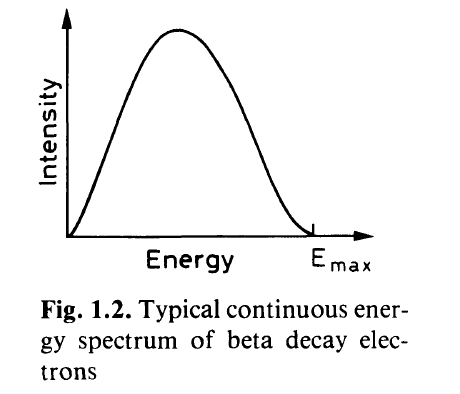
\includegraphics[width=0.45\textwidth,valign=t]{figs/q_beta.png}
  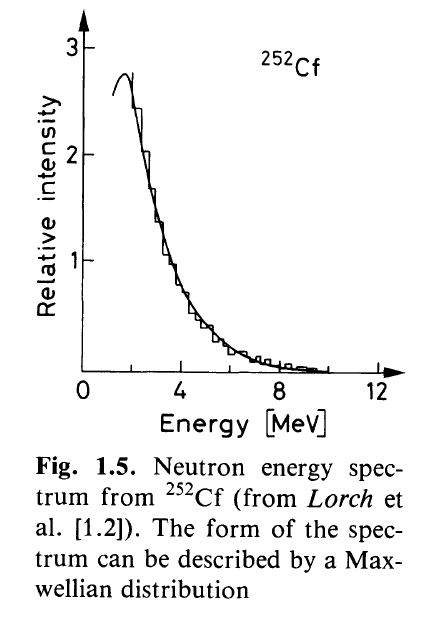
\includegraphics[width=0.45\textwidth,valign=t]{figs/q_neutron.png}
\end{center}
\end{itemize}

\section{Passage of radiation through matter}
\begin{itemize}
  \item The probability of at least one interaction over a distance $x$ is $P(x) = 1-\exp[-n\sigma x]$, where $n$ is the number density of targets
  \begin{itemize}
    \item $\Rightarrow$ mean free path $\lambda = 1/N\sigma$
  \end{itemize}
\end{itemize}
\subsection{Energy loss of heavy charged particles in matter}
\begin{itemize}
  \item Anything heavier than $m_e$
  \item Interactions are with atomic $\el$ primarily: $\sigma \sim 10^7\text{-}10^8~\ba$
  \item Either excite (soft) or eject (hard) the $\el$
  \begin{itemize}
    \item $\el$ from hard interactions can cause secondary ionization
  \end{itemize}
  \item Quantity of interest is $-\la dE/dx\ra$, assuming large fluctuations are very unlikely (untrue for $e$)
  \item Bohr's classical calculation:
  \begin{itemize}
    \item Assuming the impact parameter between the charged particle (charge $z$) moving at velocity $v$ and the $\el$ is $b$:
    \begin{align*}
      I = \frac{2ze^2}{bv} &\Rightarrow \Delta E(b) = \frac{I^2}{2m_e} = \frac{2z^2e^4}{m_ev^2b^2}\\
      \Rightarrow - \dd{E}{x} & = \frac{4\pi z^2 e^4}{m_ev^2}N_e \ln \frac{\gamma^2 mv^3}{ze^2\nubar} \numberthis
    \end{align*}
    \item where $\nubar$ is the average frequency of bound state electrons. 
    \item The value of $dE/dx$ is gotten by integrating over a reasonable range for $b$ 
    \item Valid for very heavy particles (like $\alpha$), but not for protons, etc, because quantum effects
  \end{itemize}
  \item Bethe-Bloch:
  \begin{itemize}
    \item 
    \begin{equation}
      - \left\la \frac{dE}{dx} \right\ra \propto \rho \frac{Z}{A}\frac{z^2}{\beta^2} \left[\ln \left( \frac{2 m_e \gamma^2 \beta^2 W_{\max}}{I^2}\right) - 2\beta^2 - \delta - 2 \frac{C}{Z} \right]
    \end{equation}
    where:
    \begin{itemize}
      \item $W_\text{max}$ is the maximum energy transfer kinematically allowed
      \item $I$ is the mean excitation potential (material-dependent)
      \item $\delta$ is the density correction (at high $\beta$). Corrects for the charged particle polarizing the medium as it travels through (stronger effect for high density). This cancels the quadratic rise from the $\beta^2$ term
      \item $C/Z$ is the shell-effect. Corrects for case when the incident particle is slow relative to the electron orbital velocity
    \end{itemize}
    \item Important features:
    \begin{itemize}
      \item Minimum ionizing particle occurs at $\beta \sim 0.96 \Rightarrow \gamma \sim 3.6$ (independent of the particle)
      \item $dE/dx$ goes down as a function of $\beta$ at low energies: slow particles feel atomic electric field for longer
      \item But then the $\beta^2$ relativistic effect causes a rise at high energies: Lorentz contraction of $\E$-field makes transverse component (wrt particle motion) larger. 
      \item The quadratic rise in $\beta$ is canceled by the $\delta$ ionization term. Cancellation is stronger for denser materials.
    \end{itemize}
    \begin{center}
      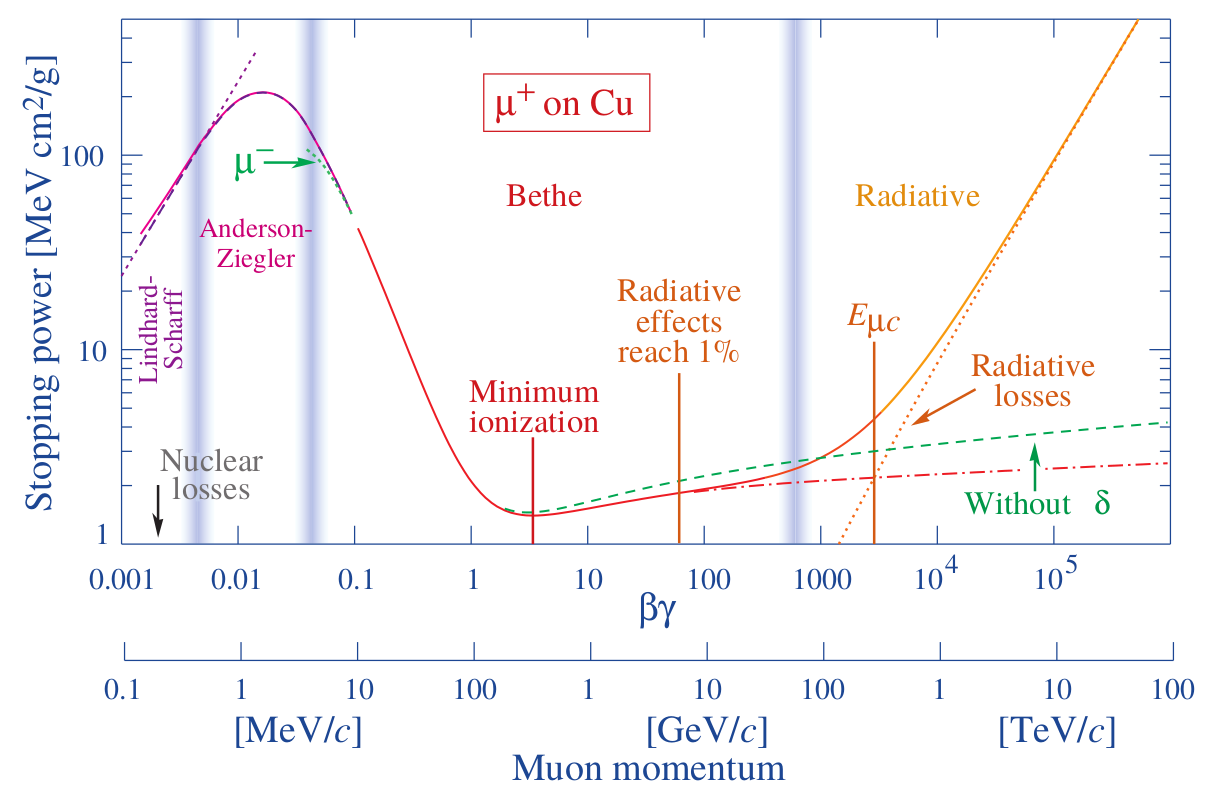
\includegraphics[width=0.8\textwidth]{figs/dEdx_bbPDG.png}
      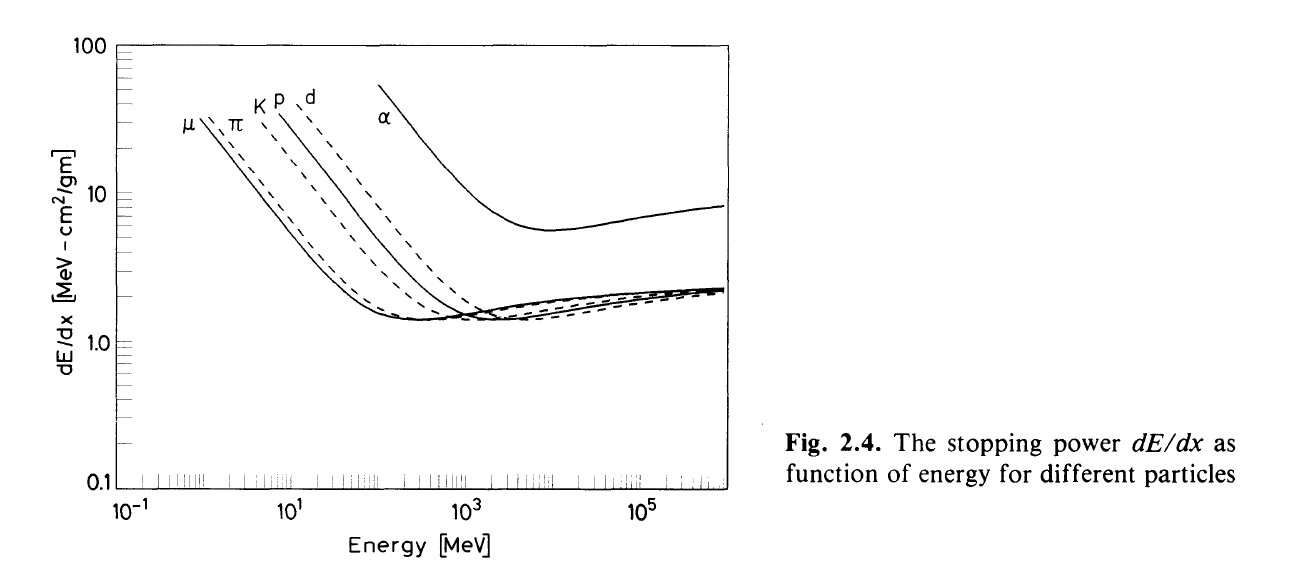
\includegraphics[width=0.8\textwidth]{figs/dEdx_bethebloch.png}
    \end{center}
    \item Note that the particle is more ionizing at low $E$ \thus more ionization occurs at end of path
    \embedimgw{figs/dEdx_bragg.png}{0.8}
    \item For a fixed medium:
    \begin{itemize}
      \item $\dd{E}{x} = z^2 f(\beta)$
      \item \thus if $\dd{E}{x}$ is known for one particle, it is known for all particles (just have to scale $z^2$ and calculate new $\beta$ as a function of energy, mass)
    \end{itemize}
  \end{itemize}
\end{itemize}

\subsection{Cerenkov radiation}
\begin{itemize}
  \item Speed of light in medium is $c/n$
  \item If $\beta>1/n$, a cone of light is observed at an angle $\theta_C$
  \item $\cos\theta_C = (\beta n(\nu))\inv$ ($\nu$ is the frequency of the radiation)
  \item The energy loss is:
  \begin{gather*}
    - \dd{E}{x} = z^2 \frac{\alpha \hbar}{c} \int d\nu \left[\nu \left(1-(\beta n(\nu))^{-2}\right) \right]\\
    \Longleftrightarrow \\
    \frac{d^2N_\gamma}{d\nu dx} = \frac{z^2\alpha}{c}\left(1-(\beta n(\nu))^{-2}\right) \numberthis
  \end{gather*}
\end{itemize}

\subsection{Interactions of electrons/positrons in matter}
\begin{itemize}
  \item Bremsstrahlung becomes dominant at $E>E_c~\sim\ord{10}~\mev$. Below this, collisions are dominant (described by Bethe-Bloch)
  \item Bremsstrahlung cross-section is $\propto (e^2/m)^2$ \thus for particles with high $m$, bremsstrahlung doesn't become relevant until very very high $E$
  \begin{itemize}
    \item Kicks in at lower $E$ for $e^\pm$
  \end{itemize}
  \embedimgw{figs/dEdx_electrons.png}{0.8}
  \item $E_c$ is defined as the energy at which $dE/dx$ due to collision and brem are the same. An empirical formula is:
  \begin{equation}
    E_c = \frac{800~\mev}{Z+1.2}
  \end{equation}
  \item For muons, $E_c$ is $\sim \tev$ (for low $Z$) to $\sim 100~\gev$  (high $Z$)
  \item Radiation length: distance over a particle's energy is reduced by $1/e$. Call it $\lrad$
  \begin{itemize}
    \item $E=E_0 \exp[-x/\lrad]$
  \end{itemize}
  \begin{center}
    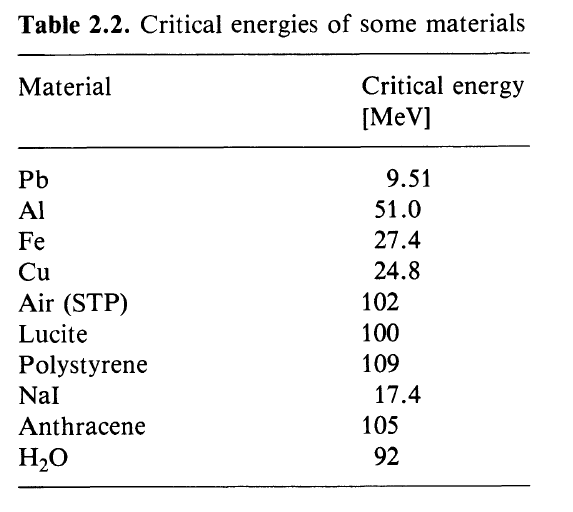
\includegraphics[width=0.45\textwidth,valign=t]{figs/ecrit_table.png}
    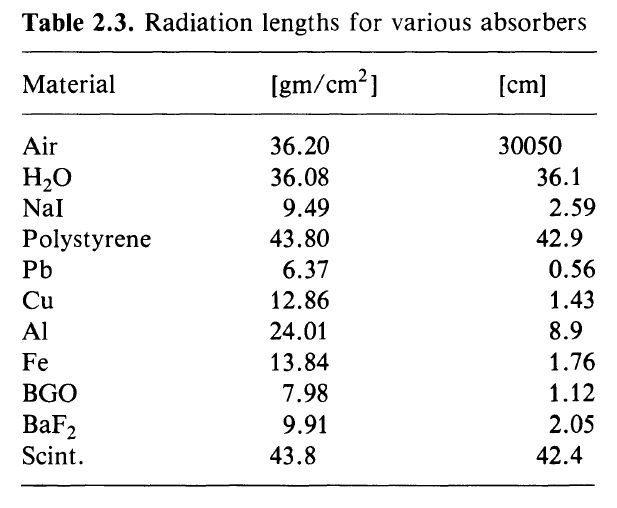
\includegraphics[width=0.45\textwidth,valign=t]{figs/radlength_table.png}\\
    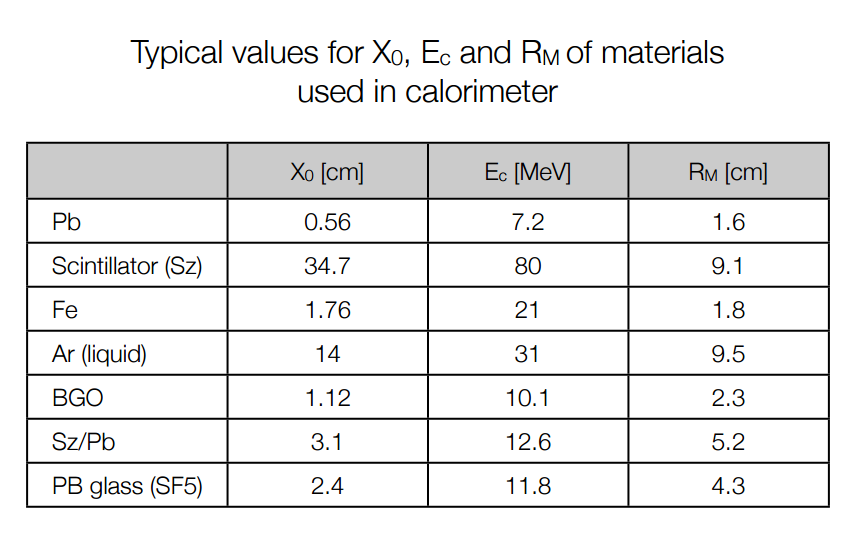
\includegraphics[width=0.6\textwidth,valign=t]{figs/tab_ecritxo.png}
  \end{center}
  \item Because of low mass, variance in $dE/dx$ is larger for $e^\pm$ than for heavier particles (long tail from large energy transfers)
\end{itemize}

\subsubsection{Multiple Coulomb scattering}
\begin{itemize}
  \item Elastic scattering off nuclei
  \item Very little energy loss since $m_{A} \gg m$ typically
  \item Rutherford formula:
  \begin{equation}
    \dd{\sigma}{\Omega} = z^2Z^2 \left(\frac{\alpha\hbar c}{T}\right)^2 \frac{1}{\sin^4(\theta/2)}
  \end{equation}
  \begin{itemize}
    \item $T$ is the kinetic energy
    \item Largest probability for small deflections
  \end{itemize}
  \item Multiple ($N_\text{scatt.}>20$) scatterings can be treated statistically
  \begin{itemize}
    \item Assume $P(\theta)$ is Gaussian centered at $0$ (this ignores large deflections in the tails)
    \item $\la \theta^2\ra \sim 10^{-3}~\text{rad}^2$ for typical materials
    \item Not valid for $e^{\pm}$ which have low mass \thus large deflections (like backscattering) possible
  \end{itemize}
\end{itemize}

\subsection{Interaction of photons in matter}

\subsubsection{Photoelectric effect}
\begin{itemize}
  \item $\gamma$+atom $\rightarrow$ ion+$\el$
  \item $E_e$ = $h\nu - \phi$, $\phi$ is the binding energy
  \item $\sigma$ decreases as $h\nu$ increases, with a jump up when $h\nu$ reaches a shell binding energy
  \item $\sigma\sim \ord{10^{-1}-10^{4}}~\ba$ and is proportional to $Z^\alpha$, for $\alpha=4-5$ (exact value is a function of $h\nu$)
\end{itemize}
  \embedimgw{figs/sigma_pe.png}{.8}

\subsubsection{Compton scattering}
\embedimgw{figs/compton_feynman.png}{0.4}
\begin{itemize}
  \item Kinematics
    \begin{gather*}
      \lambda'-\lambda = \frac{1}{\nu'} - \frac{1}{\nu} = \frac{h}{m_e} \left(1-\cos\theta\right)\\
      \cot\phi = \left(1+\frac{h\nu}{m_e}\right)\tan \frac{\theta}{2}
    \end{gather*}
  \item Klein-Nishina:
    \begin{align*}
      \dd\sigma\Omega &= \frac{\alpha^2}{2m_e^2} \left(\frac{\nu'}{\nu}\right)^2 \left[\frac{\nu'}{\nu}+\frac{\nu}{\nu'} - \sin^2\theta\right] \numberthis \\
       \sigma & \sim 10^{-4} - 10^0~\ba
    \end{align*}
  \item Can define $\sigma_S$ ($\sigma_A$) as the cross-section of scattered (absorbed) energy:
    \begin{equation}
      \dd{\sigma_S}{\Omega} = \frac{h\nu'}{h\nu}\dd\sigma\Omega, \quad \sigma_A = \sigma-\sigma_S
    \end{equation}
    \embedimgw{figs/sigma_compton.png}{.8}
  \item Can also define $d\sigma/dT$, where $T$ is the kinetic energy of $\el$:

  \begin{minipage}{.4\textwidth}
    \embedimgw{figs/dEdT_compton.png}{.8}
  \end{minipage}
  \begin{minipage}{.6\textwidth}
      $0 < T < T_\text{max}$, where $T_{\max}$ is the max allowed recoil energy:
      \begin{equation}
        T_{\max} = h\nu \frac{2\xi}{1+2\xi},~\xi = \frac{h\nu}{m_e}
      \end{equation}
  \end{minipage}
\end{itemize}

\subsubsection{Pair production}
\begin{itemize}
  \item $\gamma\rightarrow \el\pos$
  \item Mean free path: $\lambda_\text{pair} = \frac{9}{7}L_\text{rad}$, where $L_\text{rad}\sim \ord{10}~\cm$ is for electrons
  \embedimgw{figs/sigma_pair.png}{.4}
\end{itemize}

\subsubsection{Photon interaction summary}

\embedimgw{figs/sigma_photonInclusive.png}{.9}

\subsubsection{EM showers}
\begin{itemize}
  \item $\gamma\rightarrow\el\pos$, $e^\pm\rightarrow e^\pm+\gamma$, $\gamma\rightarrow\el\pos\cdots$
  \item Assuming the radiation lengths are $L_\gamma\sim L_e$:
  \begin{itemize}
    \item $N_\text{particles}\sim 2^{x/L}$
    \item $E(x)\sim E_0/2^{x/L}$, where $E$ is the energy per particle in the shower at distance $x$
    \item Obviously has to truncate when $E(x)\leq m_e$, but actually stops at $E<E_c$ (no more brem)
    \item Let $t=x/L$. Then, $t_{\max} = \ln(E_0/E_c)/\ln2$ and $N_{\max}\approx E_0/E_c$
    \begin{itemize}
      \item Need to add correction for particle that induces shower: $t_{\max} = \log_2 (E_0/E_c) - C$
      \item $C = 0.5$ if $\gamma$, else $C = 1$ 
    \end{itemize}
  \end{itemize}
\end{itemize}

\subsection{Interactions of neutrons in matter}
\begin{itemize}
  \item High energy neutrons: $E>100~\mev$
  \item Fast: $\ord{100}~kev < E < \ord{10}~\mev$
  \item Epithermal: $\ord{0.1}~\ev < E <\ord{100}~\kev$ (where nuclear resonances occur)
  \item Thermal: $E\sim 1/kT \approx 1/40~\ev$
  \item Ultracold: $E<0.001~\ev$
\end{itemize}
\subsubsection{Mechanisms of interaction}
\begin{itemize}
  \item $A+n\rightarrow A+n$: dominant for $\mev$ neutrons (elastic)
  \item $A+n\rightarrow A^*+n'$, $A+n\rightarrow B+2n',\dots$
  \begin{itemize}
    \item Neutron must be $> 1~\mev$ to excite the nucleus
    \item Inelastic
  \end{itemize}
  \item Radiative $n$ capture: $n+(Z,A)\rightarrow \gamma+(Z,A+1)$
  \begin{itemize}
    \item $\sigma \sim 1/v$, so dominant at low energies
    \item There can be resonance peaks
  \end{itemize}
  \item $A+n\rightarrow B + p/d/\alpha/t/\alpha p/\cdots$
  \begin{itemize}
    \item Typically $\ev-\kev$
    \item $\sigma\sim 1/v$
  \end{itemize}
  \item Fission (more likely at low [thermal] energies)
  \item High energy hadron shower
  \begin{itemize}
    \item Similar to EM shower
    \item $E > 100~\mev$
  \end{itemize}
\end{itemize}
\subsubsection{Neutron moderation}
\begin{itemize}
  \item Neutrons bounce around matter, slowing down until at thermal eq. w/ matter
  \begin{itemize}
    \item Unlikely to be captured by nucleus (or cause fission) at high energies because $\sigma\sim 1/v$ for these processes
  \end{itemize}
  \item Energy of scattered neutron:
  \begin{equation}
    \left(\frac{A-1}{A+1}\right)^2 E_0 < E' <E_0
  \end{equation}
  which implies low $A$ is better for absorbing energy
\end{itemize}

\section{General characteristics of detectors}
\begin{itemize}
  \item Sensitivity to signal is a function of many things:
  \begin{itemize}
    \item $\sigma$ of ionizing reactions in the detector
    \item Detector mass
    \item Material surrounding sensitive volume of detector
  \end{itemize}
  \item Two continuous responses are considered resolved if separated by a distance greater than the FWHM
  \item Error is Poissonian for detectors that collect \emph{some} of the particle's energy
  \begin{itemize}
    \item Error is smaller for detectors that \emph{stop} the particle, since each interaction is not independent
  \end{itemize}
  \item Define $J=E/W$, so the energy variance is $\sigma^2=FJ$
  \begin{itemize}
    \item $W=$energy lost per ionization in detector
    \item $F=$Fano factor
    \begin{itemize}
      \item $F=1$ \thus purely Poissonian (e.g. scintillators in which only part of the energy is deposited)
      \item $F<1$ \thus better (semiconductors, gases, scintillators which stop the particle)
    \end{itemize}
    \item Resolution can be defined two ways:
    \begin{itemize}
      \item $\text{FWHM} = 2.35 \dfrac{\sigma}{J} = 2.35\sqrt{\dfrac{FW}{E}}$
      \item Deviation divided by mean: $\dfrac{\sigma}{\mu} = \dfrac{\sigma}{J} = \sqrt{\dfrac{FW}{E}}$
    \end{itemize}
  \end{itemize}
\end{itemize}

\section{Ionization detectors}
\subsection{Types of gaseous ionization detectors}
\embedimgw{figs/gasionization.png}{.8}
\begin{itemize}
  \item Filled with a noble gas
  \item Radial $\E$-field from anode wire to cathode ($\propto 1/\ln(b/a)$, where $a$ is the wire radius and $b$ is the chamber radius)
  \item Radiation creates $\el$/ion pairs in tube
  \begin{itemize}
    \item If the radiation is charged, this occurs through ionization
    \item If neutral, it occurs through secondary ionization (i.e., $\gamma,n$ ejects an $\el$ from an atom, which then ionizes the gas)
    \item Number of pairs is $\propto E$
    \item $\el\rightarrow$anode, ions$\rightarrow$cathode
    \item Observed signal is a function of $V_0$:
    \embedimgw{figs/ionization_voltage}{0.8}
  \end{itemize}
\end{itemize}
\subsubsection{Resistive plate chamber}
\begin{itemize}
  \item Two resistive plates with small gas gap ($\sim 2~\mm$) and large voltage on electrodes outside of the plates ($\sim 10~\text{kV}$)
  \item Advantage: good time resolution $\sim 50-100~\ps$
  \item Disadvantage: bad signal quality, dark rates
\end{itemize}
\subsubsection{Ionization chamber}
\begin{itemize}
  \item Number of $\el$/ion pairs produced is equal to number of ionizations by particle
  \item Current is typically quite low
  \item Can be used for experiments with large radiation fluxes
\end{itemize}
\subsubsection{Proportional counter}
\begin{itemize}
  \item $\el$ from primary ionization drifts towards anode ($v\sim \mum/\ns$)
  \item $\E$-field is strong enough close to the anode that $\el$s from ionization are accelerated and cause secondary ionizations
  \item These secondary ionization $\el$s can also create tertiary ionizations, and so forth
  \item Occurs in the ``avalanche region'' close to the anode (since $|\vec E(r)|\propto 1/\ln(r/a)$), typically $r-a \lesssim 10~\mum$
  \item Up to $10^6$ amplification
\end{itemize}
\subsubsection{Geiger-M\"uller counter}
\begin{itemize}
  \item $\Delta V$ is so high that an ionization sparks multiple avalanches along entire length of anode
  \begin{itemize}
    \item $\el$s from primary ionization are accelerated so strongly that when they hit an atom, they ionize it but also put the atom in an excited state
    \item When the atom de-excites, it releases a $\gamma$, which initiates its own avalanche
    \item Output current is independent of $E$
    \item Need a quenching gas to absorb $\gamma$s and shorten the signal pulse
  \end{itemize}
  \item Obviously only useful for counting number of incident particles
  \item If $V_0 > 1~\text{kV}$, you get spontaneous breakdown of the gas, and it is no longer useful
\end{itemize}

\subsection{Ionization and transport in gas}
\begin{itemize}
  \item Ionization mechanisms (assuming $\psi$ is some charged particle):
  \begin{itemize}
    \item $\psi+X\rightarrow\psi+X^*$ is a resonant process
    \begin{itemize}
      \item In noble gases, $\sigma\sim 10^7~\ba$
    \end{itemize}
    \item $\psi+X \rightarrow \psi+X^++\el$ is not resonant
    \begin{itemize}
      \item $\sigma\sim 10^8~\ba$
      \item Higher energy threshold than excitations (need to overcome valence binding energy)
    \end{itemize}
  \end{itemize}
  \item In general, $\sigma$ is higher for low-energy transfers, so excitations dominate ionizations
  \item $\el$/ion pairs produced by $\psi$ can also create secondary $\el$/ion pairs if energetic enough
  \begin{itemize}
    \item Process repeats until $E_{\el}<$ionization threshold
  \end{itemize}
\end{itemize}
\subsubsection{Mean number of $\el$/ion pairs}
\begin{itemize}
  \item Note that the number of pairs is not equal to (energy lost)/(ionization energy), because some energy is lost through excitation of atoms
  \item In noble gases, 1 $\el$/ion pair produced corresponds to $\sim30~\ev$ energy lost
  \item For gaseous detectors, the Fano factor is typically $\sim 0.2$
\end{itemize}
\subsubsection{Recombination and $\el$-attachment}
\begin{itemize}
  \item These processes eat up $\el$/ion pairs before detection
  \item Recombination: if $\psi+X\rightarrow \psi+X^++\el$, then we can have $X^++\el \rightarrow X+\gamma$
  \begin{itemize}
    \item Similarly, if two ions exist in the gas: $X^++Y^- \rightarrow XY+\gamma$
  \end{itemize}
  \item Electron attachment: capture by electronegative atoms: $\el+Y \rightarrow Y^- + \gamma$
\end{itemize}
\subsubsection{Diffusion}
\begin{itemize}
  \item In principle, a charged particle in a detector will follow the $\E$-field lines
  \item But, it can be knocked about through elastic collisions with atoms
  \item Problem for detectors in which electrons must drift very far
  \item One way to minimize the effect is to add a parallel $\B$-field (so that if a particle is knocked off the field line, it remains in a tight helix). This is done in TPCs
\end{itemize}

\subsection{Avalanche multiplication}
\embedimg{figs/avalanche.png}
\begin{itemize}
  \item The initial $\el$ has high energy and causes secondary, tertiary, etc ionizations
  \item $\el$s move much faster than ions, giving the charge distribution a liquid drop shape
  \item Let $\lambda$ be the mean free path of an $\el$ causing secondary ionization
  \begin{itemize}
    \item $\alpha = \lambda\inv$ is the prob. of ionization/unit length
    \begin{equation}
      dn = n\alpha dx
    \end{equation}
    where $n$ is the number of free $\el$. Then:
    \begin{equation}
      n = n_0 e^{\alpha x}
    \end{equation}
    where $n_0$ is the number of primary ionizations
    \item $e^{\alpha x}$ is the proportionality factor in prop. counters
  \end{itemize}
  \item Above calculation assumes a constant $\E$-field \thus constant $\alpha$
  \begin{itemize}
    \item More generally:
    \begin{equation}
      e^{\alpha x}\rightarrow \exp \left[\int_{r_1}^{r_2} dx~\alpha(x)\right]
    \end{equation}
  \end{itemize}
\end{itemize}

\subsection{Pulse formation and shape}
\begin{itemize}
  \item Consider a cylindrical proportional counter as an example
  \item Consider the counter as a coax capacitor with capacitance/unit length $C$
  \begin{itemize}
    \item If a charge $q$ moves by $dr$, then 
    \begin{equation}
      dW = q\dd{\phi}{r} dr
    \end{equation}
    where $W$ is the system energy and $\phi$ is the electric potential
    \item For a capacitor of length $L$, $W = \frac{1}{2}LCV_0^2$, so
    \begin{equation}
      dW = LCV_0 dV
    \end{equation}
    \item Equating:
    \begin{equation}
      dV = \frac{q}{LCV_0}\phi'(r) dr
    \end{equation}
    \item That is, the motion of $q$ by $dr$ induces a measurable change in the potential 
  \end{itemize}
  \item \thus observed signal is \emph{not} charges collecting on the wire/wall, but an induced voltage change due to moving charges
  \item The total induced voltage change for a particle starting a distance $r'$ from the wire is:
  \begin{equation}
    \int dV = \int_{a+r'}^{R} dr~\frac{q}{LCV_0}\phi'(r)
  \end{equation}
  where $R = a$ ($R=b$) for $\el$ (ions). 
  \begin{itemize}
    \item Avalanches only occur when the $\E$-field is very high (close to the anode), so typically $r\sim\ord(1)~\mum$ ($a\sim\mum,b\sim\mm$)
    \item i.e. $b-(a+r')\gg r'$ \thus pulse is primarily caused by motion of positive charges
    \item For many (but not all!) types of prop. counters, can ignore signal from $\el$
  \end{itemize}
  \item In the following figure, time starts with the beginning of the avalanche (drift time is ignored)
  \embedimgw{figs/propcounter_pulseshape.png}{.8}
\end{itemize}

\subsection{Multiwire proportional chamber}
\embedimgw{figs/mwpc_config.png}{.8}
\begin{itemize}
  \item Cathode planes are separated by $\sim 10~\mm$ and the wires are spaced $\sim 2~\mm$ apart
  \begin{itemize}
    \item Spatial resolution is $\sim 1/2$ of wire spacing
  \end{itemize}
  \item The efficiency of a particle creating a signal is typically $\sim 99\%$
  \item Free $\el$/ions drift towards nearest anode wire/cathode wall
  \item Upon getting close to the anode, $\el$ can induce avalanche
  \item Ions from avalanche induce negative voltage difference on anode (same as proportional counter)
  \item Also induces a small \emph{positive} signal on adjacent anodes
  \item Can align many MWPCs (with alternating layers at right angles) to determine trajectory
  \begin{itemize}
    \item With sufficiently many such layers, can get 3D particle trajectory reconstruction
  \end{itemize}
  \embedimgw{figs/mwpc_xy.png}{.8}
  \item Since each anode wire is a separate detector, MWPCs can detect multiple particles, as long as they do not overlap
  \item Magic gas: $75\%$ Ar, $24.5\%$ isobutane, $.5\%$ freon \thus gains up to $\sim 10^7$
  \begin{itemize}
    \item Argon is used because noble gases require smallest $\E$-field for avalanche
    \item Above gains of $\sim10^3$, argon atoms will become excited and then de-excite by releasing a $\gamma$ \thus can release photoelectric $\el$ in cathode
    \item Add a quenching gas (isobutane) to absorb $\gamma$s and dissipate energy thermally
    \item Freon is added to kill any remaining dark current (i.e. electrons escaping from cathode due to high $\E$-field). Freon is very electronegative and therefore can capture low-energy $\el$s
  \end{itemize}
  \item If magic gas is used:
  \begin{itemize}
    \item The signals are saturated and independent of energy \thus can be used for position tracking
    \item High gain \thus signal from $\el$s is measurable. This is much faster than the ion signal, giving better timing resolution $\sim25\text{-}30~\ns$
  \end{itemize}
  \item Multiple firings 
  \embedimgw{figs/mwpc_multiple.png}{.8}
  \begin{itemize}
    \item The first and last ionizations in the diagram above will give delayed signals (wrt the second and third ionizations) because of the $\el$ drift time
    \item Typically use this timing info to get the signal localized to one or two anode wires
  \end{itemize}
\end{itemize}

\subsection{Drift chamber}
\begin{itemize}
  \item Similar to proportional counter. Uses many ``field wires'' held at constant potential to ensure uniform $\E$-field
  \item Uniform $\E$-field \thus constant drift velocity
  \embedimgw{figs/drift1.png}{.8}
  \item Operation:
  \begin{itemize}
    \item Particle sets off scintillator. Timer starts
    \item Particle ionizes an atom in chamber. \el drifts to anode
    \item \el reaches (near) anode, inducing a signal through avalanche. Timer stops
    \item Using $\Delta t$ and constant drift velocity of $\el$, position in $z$ can be determined
  \end{itemize}
  \item Spatial resolution is now determined by timing resolution of scintillator and anode signal
  \begin{itemize}
    \item \thus no longer need high wire density (like MWPCs)
  \end{itemize}
  \item Max counting rate is $\sim 10^4$/(s$\cdot$mm)/wire
  \begin{itemize}
    \item Same as MWPCs, but fewer wires \thus smaller flux can be handled
  \end{itemize}
  \embedimgw{figs/drift2.png}{.8}
  \item Cylindrical drift chambers used at collider detectors
  \item Drift chamber is much more sensitive to gas composition, pressure, impurities, because all these things affect constant drift velocity assumption
  \item Correction needs to be made to account for presence of a $\B$-field
  \item Drift velocity of $\el$ is $\sim \ord{10}~\mum/\ns$ in Ar
  \item Higher drift velocity \thus lower uncertainty from diffusion
\end{itemize}

\subsection{Time projection chamber}
\begin{center}
  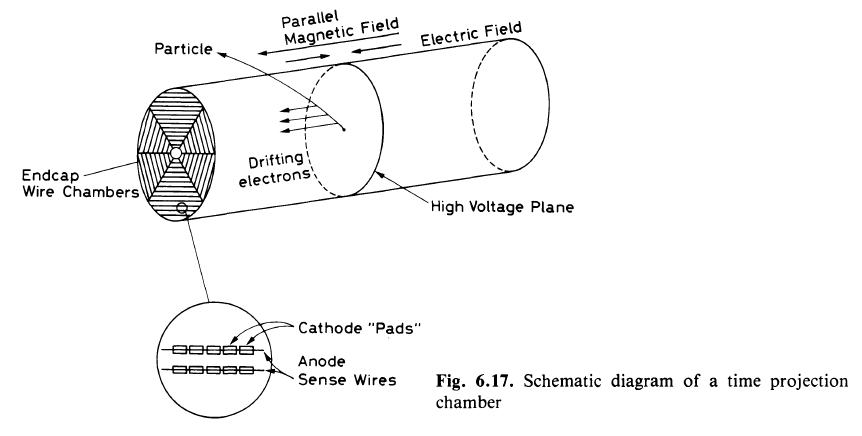
\includegraphics[width=0.6\textwidth,valign=t]{figs/tpc1.png}
  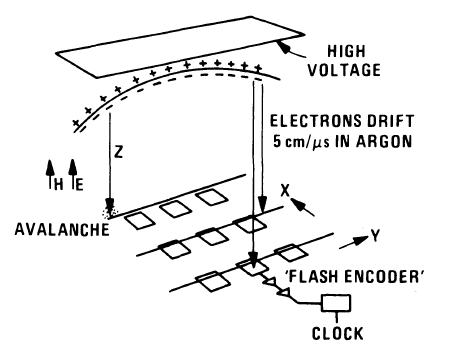
\includegraphics[width=0.38\textwidth,valign=t]{figs/tpc2.png}
\end{center}
\begin{itemize}
  \item Combines principles of a MWPC and drift tube, as well as giving info on particle momentum and $dE/dx$
  \item Constant \E-field \thus electron drift velocity is constant
  \item \B-field has two purposes:
  \begin{itemize}
    \item Curves tracks of charged particles
    \item Ensures \el diffusion (multiple scattering) is always helical towards endcap of TPC
  \end{itemize}
  \item 3D reconstruction:
  \begin{itemize}
    \item 1D from which anode wire gets a signal
    \item 1D from which cathode pads get charge on them
    \item 1D from drift time
  \end{itemize}
  \item Typically add a grid held at ground potential right before endcap
  \begin{itemize}
    \item Traps positive ions before they drift back to central cathode
  \end{itemize}
  \item Charge/signal on cathode pads/anode wires is $\propto$ energy of drift \el \thus gives $dE/dx$ of particle
  \item Curvature of charged particle gives the momentum
  \item Anode wire spacing is $\sim1~\cm$
  \item Scintillation (i.e. for LAr TPC)
  \begin{itemize}
    \item Liquid argon better for number of reasons
    \begin{itemize}
      \item Higher density than gas (good for low $\sigma$ interactions like $\nu N$)
      \item Scintillator
      \item Very low electronegativity
    \end{itemize}
    \item If the gas (or liquid) is a scintillator, can add photodetectors to measure position along $z$ axis
    \item Can use this info to know where the ionization occured (instead of relying on drift time)
  \end{itemize}
\end{itemize}

\section{Scintillators}
\begin{itemize}
  \item Particle excites an atom/molecule, which then de-excites by releasing a $\gamma$
  \item Emitted light is picked up by a photodetector
  \item Features
  \begin{itemize}
    \item Above energy threshold, scintillator response is $N_\gamma \propto E$. Since photomultipliers have $N_e\propto N_\gamma$, the total response is linear in $E$
    \item Very short deadtime, very fast response
    \item Can distinguish particle type based on pulse shape
  \end{itemize}
  \item If $N(t)$ is the number of photons emitted at time $t$, it can be approximated as the sum of a fast and slow components:
  \begin{equation}
    N = A\exp \left[-\frac{t}{\tau_f}\right] + B\exp \left[-\frac{t}{\tau_{s\vphantom{f}}}\right]
  \end{equation}
  \embedimgw{figs/scint_response.png}{.8}
  The values of $A$ and $B$ depend on the material and particle type (can be used for particle ID)
  \item Note that the above formula ignores the rise time (typically very short relative to the decay, so can be ignored).
  \item Desirable features:
  \begin{itemize}
    \item High efficiency from energy lost to radiation
    \item Transparency to radiation (so it can reach PMTs)
    \item Emission range is in operating range of PMT
    \item Short decay time $\tau$
  \end{itemize}
  \item Scintillators can be used as liquids or solids
  \item Liquid scintillators can be \emph{loaded} with other things for specific purposes (e.g. Gd or B for high neutron capture $\sigma$)
  \item Energy loss ranges from $20$ to $500$ eV/photon
\end{itemize}

\subsection{Organic scintillators}
\begin{itemize}
  \item Response time: $\leq$ few ns
  \item Molecules get excited
  \item Can have singlet ($S_0$) or triplet ($T_0$) spin ground state
  \embedimgw{figs/scint_energies.png}{0.8}
  \item $S^*$ and $S^{**}$ are electron excitations
  \item Excitation mechanism:
  \begin{enumerate}
    \item Excitation goes from $S_0$ to $S^{**}$ (or one of its vibrational excitations).
    \item Then, internal degradation to $S^{**}$ (no $\gamma$ released)
    \item Then, fluorescence  to vibrational excitation of $S_0$ (or $S_0$ itself)
    \item Since bulk of atoms are in $S_0$, photons from de-excitation to vibrational excitation of $S_0$ will not be re-absorbed
  \end{enumerate}
  \item Similar story for triplet states, but $T_0\rightarrow S_0$ is suppressed. Instead have $T_0+T_0 \rightarrow S^*+S_0~+$ phonons
  \item Liquids have a response time of $\tau\sim 3-4~\ns$
  \item Plastics 
  \begin{itemize}
    \item Organic apparently
    \item Very fast response \thus rise time cannot be ignored
    \item $\tau\sim 2-3~\ns$
  \end{itemize}
\end{itemize}

\subsection{Inorganic crystals}
\begin{itemize}
  \item Much slower $\tau\sim 500~\ns$
  \item Main advantage is high stopping power because of high density and $Z$
  \item Higher light response (2-10$\times$) than organics
  \begin{itemize}
    \item \thus better energy resolution
    \item Useful for high energy $\gamma$ or $e^\pm$
  \end{itemize}
  \item Ex: NaI or PbWO$_4$
  \item Scintillation mechanism:
  \begin{itemize}
    \item \el can be excited from valence band to excitation or conduction bands
    \item If excitation band, the \el-hole pair is in a bound state (exciton) that moves through the crystal
    \item If the exciton hits an impurity, the \el is absorbed by the impurity \thus just a hole left behind
    \item Then, an \el passing by (from a higher energy state than the hole) will fill the hole, radiating a $\gamma$ 
    \embedimgw{figs/scint_inorganic.png}{.6}
  \end{itemize}
\end{itemize}

\subsection{Gas}
\begin{itemize}
  \item Very fast $\tau\sim 1~\ns$
  \item Emits in UV range
\end{itemize}

\subsection{Pulse shape discrimination for particle ID}
\begin{itemize}
  \item Fast and slow components of decay depend on $dE/dx$
  \item The components correspond to different de-excitations with different $\Delta E$ wrt ground state
  \begin{itemize}
    \item Which excitations are populated is therefore dependent on $dE/dx$
  \end{itemize}
  \embedimgw{figs/scint_psd.png}{.6}
\end{itemize}

\subsection{Quenching}
\begin{itemize}
  \item Energy lost through de-excitations that do not radiate a $\gamma$ 
  \begin{itemize}
    \item e.g. through phonons or if the atom is ionized and the \el is recaptured later
  \end{itemize}
  \item Issue for heavy ions and $\alpha$s, which heavily ionize
  \begin{itemize}
    \item Inorganic scintillators used in this case, as they have a higher light output
  \end{itemize}
  \item Quenching \thus lower light output
\end{itemize}

\subsection{Electron detection}
\begin{itemize}
  \item ``Efficiency'' close to 100\%
  \item \emph{However} if scintillator is high $Z$, may backscatter out of detector before depositing full energy
  \begin{itemize}
    \item The 100\% therefore refers to particles being counted, not energy measurement
  \end{itemize}
  \item For low-to-medium $e^\pm$ energies, use low $Z$ organic scintillators
  \item High $Z$ inorganics good at high energy (facilitates EM shower production, depositing full energy)
\end{itemize}

\subsection{Photon detection}
\begin{itemize}
  \item Want photoelectric and pair production ($\gamma$ absorbed) to dominate Compton ($\gamma$ scattered)
  \item $\sigma_\text{photo}\propto Z^5,~\sigma_\text{pair}\propto Z^2,~\sigma_\text{Compton}\propto Z$
  \item \thus high $Z$ is better for $\gamma$s
\end{itemize}

\subsection{Neutron detection}
\begin{itemize}
  \item High energy: look for recoil in $A+n\rightarrow B+p$
  \begin{itemize}
    \item Organics good for this
    \item Pulse shape to reject $\gamma$-backgrounds
  \end{itemize}
  \item Thermal: use $A+n\rightarrow B+\gamma/\alpha$
  \begin{itemize}
    \item Use things that have neutron capture $\sigma$: Li, B, Gd
  \end{itemize}
\end{itemize}

\section{Photomultipliers}
\embedimgw{figs/pmt.png}{.6}
\begin{itemize}
  \item Operation principle:
  \begin{enumerate}
    \item $\gamma$ hits cathode, ejects \el through photoelectric effect
    \item \el is accelerated to first dynode, where it knocks out multiple \el s
    \item These are accelerated to the next dynode, each knocking out multiple \el s, and so on
    \item Number of electrons reaching anode is roughly constant per photon
  \end{enumerate}
  \item Photon must typically be in narrow energy range (i.e. from scintillator)
\end{itemize}

\subsection{Photocathode}
\begin{itemize}
  \item Quantum efficiency:
  \begin{equation}
    n(\lambda) = \frac{\text{\# of photoelectrons released}}{\text{\# of incident photons with wavelength $\lambda$}}
  \end{equation}
  \item Typically, semiconductors are used instead of metals (higher QE)
  \begin{itemize}
    \item Suppose an \el absorbs a $\gamma$ and is traveling to the surface of the material
    \item If material is metal, many interactions with free \el s \thus high $dE/dx$ \thus energy when it reaches surface may be too low to overcome potential barrier
    \item Semiconductor \el s are typically in valence bands or tightly bound \thus low $dE/dx$
  \end{itemize}
\end{itemize}

\subsection{Multiplier dynodes}
\begin{itemize}
  \item Dynodes are made of insulator coating a conductor
  \item Typically 10-14 dynodes/tube
  \item Gains of $10^6$-$10^7$
\end{itemize}

\subsection{Gain and voltage supply}
\begin{itemize}
  \item Let $V_d$ be the voltage between adjacent dynodes. The gain in $N_\el$ is $\delta = K V_d$, for some factor $K$
  \item The total gain, given $N$ dynodes, is $G = (KV_d)^N$, assuming the same $V_d$ for all dynode pairs
\end{itemize}

\subsection{Pulse shape}
\begin{itemize}
  \item We assume the input photon distribution is from a scintillator with exponentially decaying response
  \item Then, the current is also exponentially decaying: $I = dQ/dt$, $Q = N_e\propto N_\gamma$
  \embedimgw{figs/pmt_pulse.png}{.7}
\end{itemize}

\subsection{Time resolution and response}
\subsubsection{Geometry of PMT}
\begin{itemize}
  \item Electrons from different parts of the cathode take different amounts of time to reach first dynode
  \item Spread in transit time is $\Delta t\sim 0.5~\ns$. The transit time itself is $\sim 0.2$-$0.5~\ns$
  \item Above values are reached by using non-uniform \E-field between cathode and first dynode
\end{itemize}
\subsubsection{Noise}
\begin{itemize}
  \item Dark current and after pulsing
  \begin{itemize}
    \item DC is mostly from thermal noise
    \item DC is exponential in $-\phi$ (work function); materials with $\phi<0$ (good for PE effect) have high DC
    \item Two sources of after pulses:
    \begin{itemize}
      \item $\gamma$ released from dynode when \el hits. It can go back and release another \el from the cathode
      \item Ions created when \el travelling through tube hits residual gas molecules. Ion travels back to cathode, release \el
    \end{itemize}
  \end{itemize}
  \item Statistical noise
  \begin{itemize}
    \item Due to statistical nature of PE effect
    \item Fluctuations in the electron multiplier system
    \begin{itemize}
      \item Statistical fluctuations in secondary emission
      \item Difference in \el transit times between dynodes
    \end{itemize}
  \end{itemize}
\end{itemize}

\section{Semiconductor detectors}
\subsection{Basic principles}
\embedimgw{figs/bandstructure.png}{.8}
\begin{itemize}
  \item Energy ``bands'' are actually many close, discrete energy levels \thus treat them as continuous
  \begin{itemize}
    \item Arise from degenerate latice energy levels breaking into many close discrete levels (due to Pauli principle)
  \end{itemize}
  \item Below the valence band are tightly-bound \el s
  \item Conduction band: free to roam in lattice
  \item Valence band: more tightly bound to individual atoms
  \item In an insulator, the bands are far apart. Im a semiconductor, the band gap is $\sim 1~\ev$
  \item When a voltage is applied:
  \begin{itemize}
    \item Insulator: valence \el s are stuck \thus no current
    \item Metal: Thermally excited \el s are in the conduction band \thus current flows
    \item Semiconductor: only a few \el s in the conduction band, so a small current is observed. As $T\rightarrow 0$, the current decreases
  \end{itemize}
  \item Charge carriers in semiconductors
  \begin{itemize}
    \item Thermal excitation: \el jumps to conduction band, leaving hole behind
    \begin{itemize}
      \item Conduction band \el can move freely \thus one current
      \item Valence band can also move freely \thus another source of current
      \item Hole current is due to \el s moving around to fill holes
      \item In contrast, metals only have one type of current (free \el)
    \end{itemize}
    \item Number of \el/hole pairs is $\propto T^{3/2}\exp \left[-E_g/2kT\right] $, where $E_g$ is the energy gap size at 0 K
  \end{itemize}
  \item Recombination
  \begin{itemize}
    \item Process of \el+hole$\rightarrow$phonon
    \item Expect \el/hole lifetime $\sim1~\s$
    \begin{itemize}
      \item Long because in order for recombination to occur, \el and hole must be in specific energy/momentum configuration
    \end{itemize}
    \item Experimentally, find $\tau\sim 1~\mus$-$100~\mus$ \thus some other mechanism of destroying pairs
    \item Impurities can add energy levels in the energy gap
    \embedimgw{figs/impurities.png}{.7}
    \begin{itemize}
      \item These intermediate states can capture an \el and later capture a hole (or vice versa), causing recombination
      \item Very efficient process
      \item Bad for detection, as it reduces charge carrier lifetime (i.e. recomb. occurs before the charges can be collected)
      \item Detectors need $<10^{10}$ impurities/cm$^3$
    \end{itemize}
    \item Trapping
    \begin{itemize}
      \item Similar to recombination impurities, except the extra energy states are charge-specific (i.e. only \el or holes, but not both)
      \item Charge is then released after some characteristic time
      \begin{itemize}
        \item If the capture time is longer than charge collection time, signal can be lost to trapping centers
      \end{itemize}
    \end{itemize}
    \item Recomb. and trapping effects can arise from structural defects in lattice as well
  \end{itemize}
\end{itemize}

\subsection{Doped semiconductors}
\begin{itemize}
  \item A semiconductor can be doped when a lattice atom is replaced with an atom with:
  \begin{itemize}
    \item An extra \el \thus donor (n-type) impurity
    \item A missing \el \thus acceptor (p-type) impurity
  \end{itemize}
  \item For example, if the semiconductor is Si or Ge (quadravalent atoms), a donor would have 5 valence \el (e.g. P), and an acceptor would have 3 valence \el (e.g. Al)
  \embedimgw{figs/doping.png}{.8}
  \item n-type (i.e. extra \el)
  \begin{itemize}
    \item Valence band is filled up, so extra \el creates an energy level in the gap
    \item The $\Delta E$ between the impurity state and the conduction band is $\ord{0.01}~\ev$
    \item This extra \el is very easily thermally excited into conduction band \thus better conductivity
    \item Extra \el will also drop down to fill holes \thus hole current is somewhat suppressed
  \end{itemize}
  \item p-type (i.,e. missing \el)
  \begin{itemize}
    \item Essentially everything said about n-type, but $\el \longleftrightarrow~$hole.
    \item Impurity level is very close to valence band (i.e. location of hole current)
  \end{itemize}
  \item Let $p,n$ be the concentrations of positive, negative (i.e. holes, free \el) charges respectively; $N_D,N_A$ be the concentrations of donor, acceptor impurities. Then, electric neutrality implies:
  \begin{equation}
    N_D+p = N_A+n
  \end{equation}
  \item Note that donors are positively charged: extra \el is not in valence band (so it is counted as part of $n$). Inverse is true for acceptors
\end{itemize}

\subsection{The np junction and depletion zone}
\embedimgw{figs/npjunc.png}{.8}
\begin{itemize}
  \item Basic concept: p-type semiconductor next to n-type material (actual fabrication is more complicated)
  \item n- and p-sides start neutral, but then:
  \begin{itemize}
    \item \el flow from n to p, filling holes
    \item Holes from p to n, accepting \el
    \item \thus result: p-side has static negative charge; n-side has static positive charge
    \item Static charge distributions are localized near boundary
  \end{itemize}
  \item Generates an \E-field from n to p. {\bf IMPORTANT}: sign of \E-field in above diagram (from Leo) is incorrect
  \item The \E-field is equiv to a potential difference across junction ($V_0 \sim 1$ V)
  \item Non-zero \E-field pushes the energy levels up (down) on the p (n) side
  \begin{itemize}
    \item Remember: \el move against \E
    \item More negative static charges on p-side \thus \el energy levels go up
    \item More positive static charges on n-side \thus \el energy levels go down
  \end{itemize}
  \item Capacitance: the electrostatic configuration resembles a plate capacitor with $C\sim \text{pF/mm}^2$
  \item Depletion zone
  \begin{itemize}
    \item Area in which there are no free charges
    \item Depth of n- and p-sides (calculation is below):
    \begin{equation}
      x_n = \sqrt{\frac{2\epsilon V_0}{e N_D(1+N_D/N_A)}}, \quad x_p = \sqrt{\frac{2\epsilon V_0}{eN_A(1+N_A/N_D)}}
    \end{equation}
    \item \thus if one side is more heavily doped than the other, the depletion zone extends further into the lightly-doped side
    \item Depth calculation:
  \end{itemize}
\end{itemize}

\noindent Assume the charge density is constant:
\begin{equation}
  \rho(x) = \begin{cases} - eN_D & 0 < x < x_n \\ - eN_A & -x_p < x < 0 \end{cases}
\end{equation}
Charge conservation implies $x_n N_D = x_p N_A$.  Using Poisson's equation:
\begin{equation}
  \phi''(x) = -\rho(x)/\epsilon
\end{equation}
Integrating twice and choosing constants:
\begin{equation}
  \phi(x) = \begin{cases} - \frac{eN_D}{\epsilon} \left(\frac{x^2}{2}-x_n x\right) & x\in n \\ \frac{eN_A}{\epsilon} \left(\frac{x^2}{2}+x_px\right) & x\in p \end{cases}
\end{equation}
Imposing $\phi(-x_p)=0$ and $\phi(x_n)=V_0$ allows us to solve for the depths.

\subsection{Semiconductors as detectors}
\begin{itemize}
  \item Principle: constant \E-field in depletion zone carries away charges from ionizaton
  \begin{itemize}
    \item Holes go to p-side
    \item \el go to n-side
  \end{itemize}
  \item Average energy to create \el/hole pair is $3~\ev$
  \begin{itemize}
    \item Can contrast with gases $\sim30~\ev$
    \item Scintillators are $\sim300~\ev$
  \end{itemize}
  \item For light particles ($m\lesssim m_p$), energy per ionization $w$ is independent of particle type
  \begin{itemize}
    \item Therefore, given a collection efficiency $n$, particle of energy $E$, and assuming the particle is stopped in the semiconductor:
    \begin{equation}
      Q = \frac{nE}{w}
    \end{equation}
    \item Not quite true for heavier ions $\alpha,\dots$
  \end{itemize}
  \item What is measured is a voltage difference induced by charge collected $Q$ \thus $V=Q/C$
\end{itemize}

\subsubsection{Reverse bias}
\embedimgw{figs/reversebias.png}{.8}
\begin{itemize}
  \item Normal depletion zone is rather small and \E-field is relatively weak
  \item Fix both issues by adding an additional bias voltage $V_B\gg V_0$
  \item Note: $V_B$ is maintained and $V_B\gg V_0$, so changing $V_0$ due to individual ionizations is negligible
  \item Can get depletion zones of $\sim1~\mm$
\end{itemize}

\subsubsection{Detector characteristics}
\begin{itemize}
  \item Fano factor is $\sim 0.12$ \thus energy resolution for a $5~\mev$ particle is $\sim 0.07\%$
  \item Response is very fast $\sim 10~\ns$, and timing resolution can get down to $\sim 10~\ps$
  \begin{itemize}
    \item Drift time is $\sim 10~\text{ps}/\mum$ in silicon
  \end{itemize}
  \item Dimensions are typically $\sim 100~\mum$ \thus spatial resolution is dimension divided by $\sqrt{12}$
\end{itemize}

\subsection{Silicon strip detectors}
\begin{itemize}
  \item Same basic principle as the detectors described above, just in a different geometry
  \embedimgw{figs/strips.png}{.4}
  \item p-type strips embedded in n-type bulk
  \item Thickness is typically $\sim 300~\mum$. Can get much larger depletion zone
  \item Spatial resolution is better than spacing of strips: can use the amount of charge deposited on each strip to interpolate where the ionization happened
  \begin{itemize}
    \item \thus $\sigma \sim 5~\mum$ if the spacing is $20~\mum$
  \end{itemize}
\end{itemize}

\begin{appendices}
\section{Bibliography}

Leo, W. R., \emph{Techniques for Nuclear and Particle Physics Experiments}. Second Revised Edition
\vspace{5mm}

\noindent PDG Particle Review, \emph{Passage of Particles Through Matter}. 2014 edition

\end{appendices}

\end{document}
